\documentclass{article}
\usepackage{amsmath}
\usepackage{amssymb}
\usepackage[a4paper, top=25mm, bottom=25mm, left=25mm, right=25mm]{geometry}
\usepackage{pgfplots}
\pgfplotsset{compat=1.18}
\usepackage{mathtools}
\usepgfplotslibrary{polar}
\usepgfplotslibrary{fillbetween}
\usepackage{tikz}
\usetikzlibrary{arrows.meta}

\begin{document}
\pagestyle{empty}
\large

\begin{center}
2020-2021 Spring \\MAT124 Final\\(09/06/2021)
\end{center}

\noindent 1. Sketch the region corresponding to the double integral

\[\int_{-1}^2\int_{x^2}^{x+2}\,dy\,dx\]

\hfill

\noindent and reverse the order of integration.

\hfill

\noindent 2. Find the volume of the solid bounded above by the cone $z=\sqrt{x^2+y^2}$ and below by the circular region $x^2+y^2\leq4$ in the $xy$-plane.

\hfill

\noindent 3. Let $R$ be the region lying outside $r=1$ and inside $r=1+\cos\theta$.

\hfill

\noindent (i) Sketch the graph of the region $R$.

\hfill

\noindent (ii) Set up (but do not evaluate) a double integral in polar coordinates for the area of the region $R$.

\hfill

\noindent 4. Let $S$ be the portion of the surface $z=y^2$ that lies over the rectangular region in the $xy$-plane with the vertices $(0,0,0), (0,1,0), (1,1,0)$ and $(1,0,0)$.

\hfill

\noindent (i) Sketch the graph of $S$.

\hfill

\noindent (ii) Evaluate the surface area.

\hfill

\noindent 5. Evaluate $\displaystyle \iiint_E z\,dV$, where $E$ is the region bounded below by $x^2+y^2+z^2=4$ and above by $x^2+y^2+z^2=9$.

\hfill

\noindent 6. Let $S$ be the region bounded above by the paraboloid $z=1-x^2-y^2$ and below by the $xy$-plane.

\hfill

\noindent (i) Using the spherical coordinates, set up (but do not evaluate) an integral for the volume of the solid $S$.

\hfill

\noindent (ii) Using the cylindrical coordinates, set up (but do not evaluate) an integral for the volume of the solid $S$.

\newpage

\begin{center}
2020-2021 Spring Final (09/06/2021) Solutions\\
(Last update: 05/08/2025 00:46)
\end{center}

\noindent 1.

\begin{minipage}{0.45\textwidth}
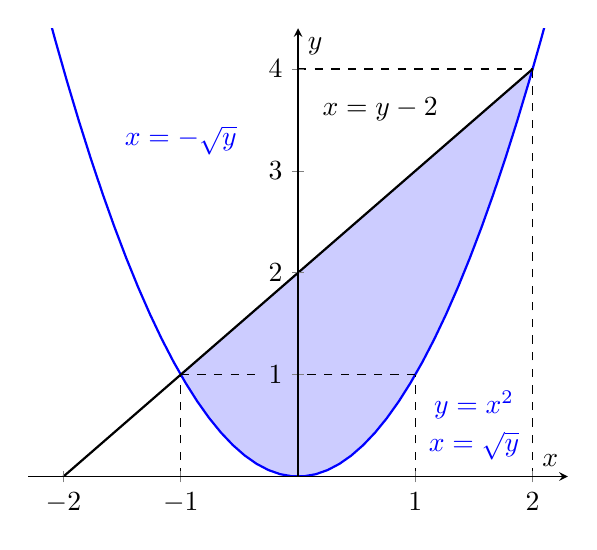
\begin{tikzpicture}
  \begin{axis}[
      axis lines = middle,
      xlabel = $x$, ylabel = $y$,
      ymin=0, ymax=4.4,
      xmin=-2.3, xmax=2.3,
      samples=100,
      clip=true,
      axis on top,
    ]
    
    \addplot [
      name path=A,
      domain=-2:2,
      draw=none,
    ] {x^2};

    \path[name path=B] (axis cs:-1,1) -- (axis cs:2,4);

    \addplot [
      fill=blue!20,
      draw=none,
    ] fill between [
      of=A and B,
      soft clip={domain=-1:2},
    ];
    
    \addplot[blue, thick] {x^2};
    \addplot[black, thick] coordinates {(-2,0) (2,4)};
    \draw[dashed] (axis cs:-1,1) -- (axis cs: -0.3,1);
    \draw[dashed] (axis cs:1,1) -- (axis cs: 0,1);
    \draw[dashed] (axis cs:2,0) -- (axis cs: 2,4);
    \draw[dashed] (axis cs:-1,0) -- (axis cs: -1,1);
    \draw[dashed] (axis cs:1,0) -- (axis cs: 1,1);
    \draw[dashed] (axis cs:0,4) -- (axis cs: 2,4);
    \node[blue] at (axis cs: 1.5, 0.7) {$y=x^2$};
    \node[blue] at (axis cs: 1.5, 0.3) {$x=\sqrt{y}$};
    \node[blue] at (axis cs: -1, 3.3) {$x=-\sqrt{y}$};
    \node at (axis cs: 0.7, 3.6) {$x=y-2$};

  \end{axis}
\end{tikzpicture}
\end{minipage}
\begin{minipage}{0.5\textwidth}
\begin{equation*}
\boxed{\int_0^1\int_{-\sqrt y}^{\sqrt y}\,dx\,dy+\int_1^4\int_{y-2}^{\sqrt y}\,dx\,dy}\end{equation*}
\end{minipage}

\hfill

\noindent 2. Using polar coordinates, we can find the volume with a double integral.

\[
\begin{array}{c}
r^2=x^2+y^2\\
dA=r\,dr\,d\theta
\end{array}\quad\rightarrow\quad
\begin{array}{c}z=\sqrt{x^2+y^2}\implies z=\sqrt{r^2}\implies z=r\\[0.3cm]
x^2+y^2\leq4\,\rightarrow\,r^2\leq4\implies 0\leq r\leq 2\\[0.3cm]
0\leq\theta\leq2\pi
\end{array}
\]

\begin{align*}\text{Volume}&=\int_0^{2\pi}\int_{0}^{2}\left[r-0\right]\cdot r\,dr\,d\theta=\int_0^{2\pi}\int_{0}^{2}r^2\,dr\,d\theta=\int_0^{2\pi}\left[\frac{r^3}3\right]_{r=0}^{r=2}d\theta\\\\&=\frac83\int_0^{2\pi}\,d\theta=\boxed{\frac{16\pi}3}\end{align*}

\hfill

\noindent 3.

\hfill

\begin{minipage}{0.5\textwidth}

(i)

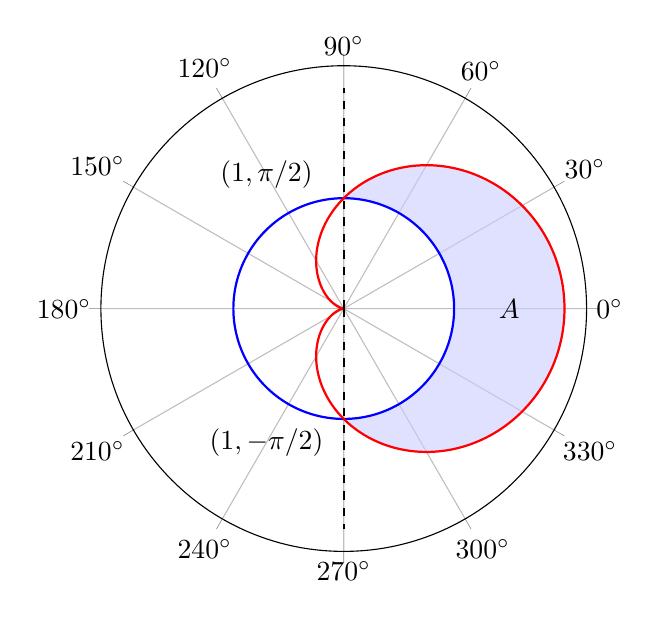
\begin{tikzpicture}
  \begin{polaraxis}[ytick=\empty, axis y line=none, scale=0.9, xticklabel=$\pgfmathprintnumber{\tick}^\circ$,]
    \addplot [
      domain=-pi/2:pi/2,
      samples=300,
      draw=none,
      name path=A,
      data cs=polarrad,
    ] {1};

    \addplot [
      domain=-pi/2:pi/2,
      samples=300,
      draw=none,
      name path=B,
      data cs=polarrad,
    ] {1+cos(deg(x))};

    \addplot [
      blue!20,
      fill opacity=0.6,
    ] fill between[of=A and B];

    \addplot [
      domain=0:2*pi,
      samples=300,
      thick,
      blue,
      data cs=polarrad,
    ] {1};

    \addplot [
      domain=0:2*pi,
      samples=300,
      thick,
      red,
      data cs=polarrad,
    ] {1+cos(deg(x))};

    \draw[black, thick, dashed] (axis cs: 90,0) -- (axis cs: 90,2);
    \draw[black, thick, dashed] (axis cs: -90,0) -- (axis cs: -90,2);

    \node at (axis cs:120,1.4) {$(1,\pi/2)$};
    \node at (axis cs:-120,1.4) {$(1,-\pi/2)$};
    \node at (0,1.5) {$A$};

  \end{polaraxis}
\end{tikzpicture}
\end{minipage}
\begin{minipage}{0.4\textwidth}
\begin{equation*}
\text{(ii)}\quad\boxed{A=\int_{-\pi/2}^{\pi/2}\int_1^{1+\cos\theta}r\,dr\,d\theta}
\end{equation*}
\end{minipage}

\newpage

\noindent 4.

\hfill

\noindent (i)

\begin{center}
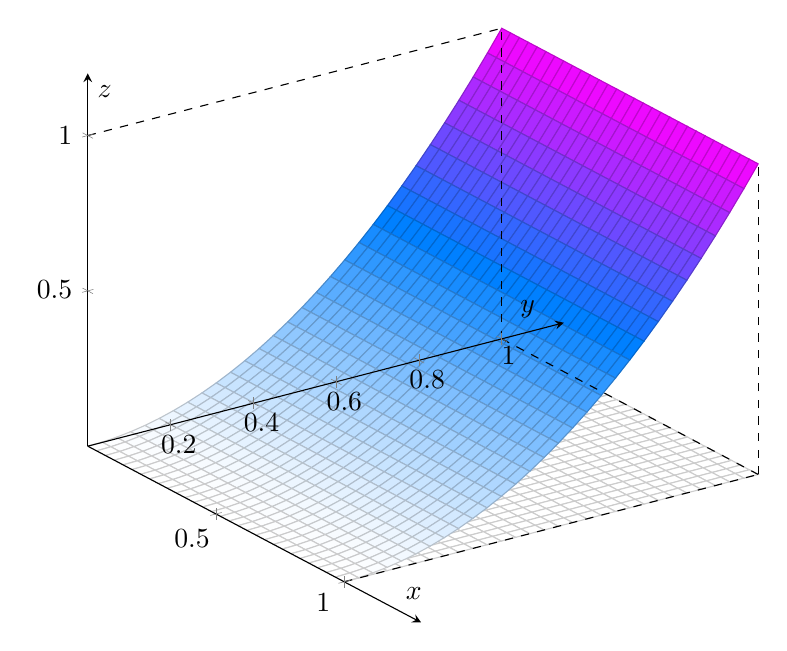
\begin{tikzpicture}
  \begin{axis}[
      view={55}{30},
      axis lines=center,
      xlabel=$x$, ylabel=$y$, zlabel=$z$,
      xmin=0, xmax=1.3,
      ymin=0, ymax=1.15,
      zmin=0, zmax=1.2,
      samples=30,
      domain=0:1,
      y domain=0:1,
      colormap/cool,
      mesh/ordering=y varies,
      scale=1.5,
      axis on top,
    ]
    
    \addplot3[surf]{0};
    \addplot3[surf]{y^2};

    \draw[dashed] (axis cs:0,1,0)--(axis cs:0,1,1);
    \draw[dashed] (axis cs:1,0,0)--(axis cs:1,1,0);
    \draw[dashed] (axis cs:0,1,0)--(axis cs:1,1,0);
    \draw[dashed] (axis cs:1,1,0)--(axis cs:1,1,1);
    \draw[dashed] (axis cs:0,0,1)--(axis cs:0,1,1);

   \end{axis}
\end{tikzpicture}
\end{center}

\hfill

\noindent (ii) Calculate the partial derivatives to find the surface area.

\begin{equation*}
z=y^2\implies\quad\frac{\partial z}{\partial x}=0,\quad \frac{\partial z}{\partial y}=2y
\end{equation*}

\hfill

\begin{align*}\text{Surface area}&=\iint_D\sqrt{1+\left(\frac{\partial z}{\partial x}\right)^2+\left(\frac{\partial z}{\partial y}\right)^2}\,dA=\int_0^1\int_0^1\sqrt{1+\left(0\right)^2+\left(2y\right)^2}\,dx\,dy\\\\&=\int_0^1\int_0^1\sqrt{4y^2+1}\,dx\,dy=\int_0^1\left[x\sqrt{4y^2+1}\right]_{x=0}^{x=1}\,dy\\\\&=\int_0^1\sqrt{4y^2+1}\,dy\:\left[y=\frac12\tan u \implies dy=\frac12\sec^2u\,du,\:\begin{array}{l}u_{\text{upper}}=\arctan2\\u_{\text{lower}}=0\end{array}\right]\\\\&=\frac12\int_0^{\arctan2}\sqrt{\tan^2u+1}\cdot\sec^2u\,du=\frac12\int_0^{\arctan2}\sec^3u\,du\end{align*}

\hfill

\noindent To evaluate the last integral, we will use integration by parts.

\begin{align*}
    w=\sec u\,&\rightarrow\, dw = \sec u\tan u \,du\\
    dz=\sec^2u\,du\,&\rightarrow\, z = \tan u
\end{align*}
\begin{align*}
\int_0^{\arctan2}\sec^3u\,du&=\tan u \cdot \sec u\,\bigg|_0^{\arctan2} -\int_0^{\arctan2} \tan^2 u\sec u\, du\\\\&= \tan u \cdot \sec u\,\bigg|_0^{\arctan2} -\int_0^{\arctan2} \frac{1-\cos^2u}{\cos^3 u}\, du\\\\&= \tan u \cdot \sec u\,\bigg|_0^{\arctan2} - \int_0^{\arctan2} \sec^3u \, du + \int_0^{\arctan2} \sec u \, du 
\end{align*}

\hfill

\noindent Notice that the integral we want to evaluate appears on the right side. After a little algebra, we can evaluate the integral.

\begin{equation*}
\int_0^{\arctan2}\sec^3u\,du=\frac12\cdot\tan u\cdot\sec u\,\bigg|_0^{\arctan2}+\frac12\cdot\int_0^{\arctan2}\sec u\,du
\end{equation*}

\hfill

\noindent The integral of $\sec u$ with respect to $u$ is as follows. One can derive it with particular methods.

\begin{equation*}\int_0^{\arctan2}\sec u \, du = \ln\left|\tan u + \sec u\right|\bigg|_0^{\arctan2}
\end{equation*}

\hfill

\noindent So, the surface area becomes as follows.

\begin{align*}\text{Surface area}&=\frac12\int_0^{\arctan2}\sec^3u\,du=\frac14\left(\tan u\cdot\sec u+\ln\left|\tan u+\sec u\right|\right)\bigg|_0^{\arctan2}\\\\&=\frac14\left[2\sec(\arctan2)+ \ln(2+\sec(\arctan2))-0\right]=\boxed{\frac14\left[2\sqrt5+\ln\left(2+\sqrt5\right)\right]}\end{align*}

\hfill

\noindent 5. By means of spherical coordinates, we can easily evaluate the integral. For spherical coordinates, we have

\[
\begin{array}{c}
z=\rho\cos\theta\\
r=\rho\sin\theta\\
x^2+y^2+z^2=\rho^2\\
dV=\rho^2\sin\phi\,d\rho\,d\phi\,d\theta
\end{array}\quad\rightarrow\quad
\begin{array}{c}
x^2+y^2+z^2=4\,\rightarrow\,\rho^2 = 4\implies \rho_{\text{min}}=2\\
x^2+y^2+z^2=9\,\rightarrow\,\rho^2 = 9\implies \rho_{\text{max}}=3\\
z\equiv\rho\cos\phi\\
0\leq\theta\leq2\pi,\quad0\leq\phi\leq\pi
\end{array}
\]

\begin{align*}
\iiint_Ez\,dV&=\int_0^{2\pi}\int_0^\pi\int_2^3\rho\cos\phi\cdot\rho^2\sin\phi\,d\rho\,d\phi\,d\theta=\frac12\int_0^{2\pi}\int_0^\pi\int_2^3\rho^3\sin(2\phi)\,d\rho\,d\phi\,d\theta\\\\&=\frac12\int_0^{2\pi}\int_0^\pi\left[\frac{\rho^4}{4}\right]_{\rho=2}^{\rho=3}\sin(2\phi)\,d\phi\,d\theta=\frac{65}{8}\int_0^{2\pi}\int_0^\pi\sin(2\phi)\,d\phi\,d\theta\\\\&=\frac{65}{8}\int_0^{2\pi}\left[-\frac12\cos(2\phi)\right]_{\phi=0}^{\phi=\pi}\,d\theta=\frac{65}{8}\int_0^{2\pi}0\,d\theta =\boxed0
\end{align*}

\newpage

\noindent 6.

\hfill

\noindent (i) For spherical coordinates, we have

\[
\begin{array}{c}
z=\rho\cos\phi\\
r=\rho\sin\phi\\
x^2+y^2+z^2=\rho^2\\
dV=\rho^2\sin\phi\,d\rho\,d\phi\,d\theta
\end{array}\quad\rightarrow\quad
\begin{array}{cc}
z=1-x^2-y^2\implies\rho\cos\phi=1-\rho^2\sin^2\phi&(1)\\[0.3cm]
\displaystyle0\leq\phi\leq\frac\pi2,\quad0\leq\theta\leq2\pi,\quad0\leq\rho\leq\rho_{\text{upper}}
\end{array}
\]

\hfill

\noindent Find $\rho_{\text{upper}}$ with equation $(1)$.

\[
\begin{array}{c}
\rho\cos\phi=1-\rho^2\sin^2\phi\implies \rho^2\sin^2\phi+\rho\cos\phi-1=0\\\\
\displaystyle \rho_{1,2} = \frac{-\cos\phi \pm\sqrt{\cos^2\phi-4\cdot\sin^2\phi\cdot(-1)}}{2\sin^2\phi}\quad\left[x_{1,2}=\frac{-b\pm\sqrt{b^2-4ac}}{2a}\right]\\\\
\displaystyle \rho>0\implies\rho_{\text{upper}}=\frac{-\cos\phi +\sqrt{\cos^2\phi+4\sin^2\phi}}{2\sin^2\phi}
\end{array}
\]

\hfill

\[\boxed{\text{Volume}=\int_0^{2\pi}\int_0^{\pi/2}\int_0^{\textstyle\frac{-\cos\phi +\sqrt{\cos^2\phi+4\sin^2\phi}}{2\sin^2\phi}}\rho^2\sin\phi\,d\rho\,d\phi\,d\theta}\]

\hfill

\noindent (ii) For cylindrical coordinates, we have

\[
\begin{array}{c}
z=z\\
r^2=x^2+y^2\\
dV=r\,dz\,dr\,d\theta
\end{array}\quad\rightarrow\quad
\begin{array}{c}
z=1-x^2-y^2\implies z=1-r^2\\
0\leq\theta\leq2\pi,\quad 0\leq r \leq1
\end{array}
\]

\[\boxed{\text{Volume}=\int_0^{2\pi}\int_0^1\int_0^{1-r^2}r\,dz\,dr\,d\theta}\]

\end{document}